% Options for packages loaded elsewhere
\PassOptionsToPackage{unicode}{hyperref}
\PassOptionsToPackage{hyphens}{url}
\PassOptionsToPackage{dvipsnames,svgnames,x11names}{xcolor}
%
\documentclass[
]{scrartcl}

\usepackage{amsmath,amssymb}
\usepackage{iftex}
\ifPDFTeX
  \usepackage[T1]{fontenc}
  \usepackage[utf8]{inputenc}
  \usepackage{textcomp} % provide euro and other symbols
\else % if luatex or xetex
  \usepackage{unicode-math}
  \defaultfontfeatures{Scale=MatchLowercase}
  \defaultfontfeatures[\rmfamily]{Ligatures=TeX,Scale=1}
\fi
\usepackage{lmodern}
\ifPDFTeX\else  
    % xetex/luatex font selection
\fi
% Use upquote if available, for straight quotes in verbatim environments
\IfFileExists{upquote.sty}{\usepackage{upquote}}{}
\IfFileExists{microtype.sty}{% use microtype if available
  \usepackage[]{microtype}
  \UseMicrotypeSet[protrusion]{basicmath} % disable protrusion for tt fonts
}{}
\makeatletter
\@ifundefined{KOMAClassName}{% if non-KOMA class
  \IfFileExists{parskip.sty}{%
    \usepackage{parskip}
  }{% else
    \setlength{\parindent}{0pt}
    \setlength{\parskip}{6pt plus 2pt minus 1pt}}
}{% if KOMA class
  \KOMAoptions{parskip=half}}
\makeatother
\usepackage{xcolor}
\setlength{\emergencystretch}{3em} % prevent overfull lines
\setcounter{secnumdepth}{5}
% Make \paragraph and \subparagraph free-standing
\ifx\paragraph\undefined\else
  \let\oldparagraph\paragraph
  \renewcommand{\paragraph}[1]{\oldparagraph{#1}\mbox{}}
\fi
\ifx\subparagraph\undefined\else
  \let\oldsubparagraph\subparagraph
  \renewcommand{\subparagraph}[1]{\oldsubparagraph{#1}\mbox{}}
\fi


\providecommand{\tightlist}{%
  \setlength{\itemsep}{0pt}\setlength{\parskip}{0pt}}\usepackage{longtable,booktabs,array}
\usepackage{calc} % for calculating minipage widths
% Correct order of tables after \paragraph or \subparagraph
\usepackage{etoolbox}
\makeatletter
\patchcmd\longtable{\par}{\if@noskipsec\mbox{}\fi\par}{}{}
\makeatother
% Allow footnotes in longtable head/foot
\IfFileExists{footnotehyper.sty}{\usepackage{footnotehyper}}{\usepackage{footnote}}
\makesavenoteenv{longtable}
\usepackage{graphicx}
\makeatletter
\def\maxwidth{\ifdim\Gin@nat@width>\linewidth\linewidth\else\Gin@nat@width\fi}
\def\maxheight{\ifdim\Gin@nat@height>\textheight\textheight\else\Gin@nat@height\fi}
\makeatother
% Scale images if necessary, so that they will not overflow the page
% margins by default, and it is still possible to overwrite the defaults
% using explicit options in \includegraphics[width, height, ...]{}
\setkeys{Gin}{width=\maxwidth,height=\maxheight,keepaspectratio}
% Set default figure placement to htbp
\makeatletter
\def\fps@figure{htbp}
\makeatother
% definitions for citeproc citations
\NewDocumentCommand\citeproctext{}{}
\NewDocumentCommand\citeproc{mm}{%
  \begingroup\def\citeproctext{#2}\cite{#1}\endgroup}
\makeatletter
 % allow citations to break across lines
 \let\@cite@ofmt\@firstofone
 % avoid brackets around text for \cite:
 \def\@biblabel#1{}
 \def\@cite#1#2{{#1\if@tempswa , #2\fi}}
\makeatother
\newlength{\cslhangindent}
\setlength{\cslhangindent}{1.5em}
\newlength{\csllabelwidth}
\setlength{\csllabelwidth}{3em}
\newenvironment{CSLReferences}[2] % #1 hanging-indent, #2 entry-spacing
 {\begin{list}{}{%
  \setlength{\itemindent}{0pt}
  \setlength{\leftmargin}{0pt}
  \setlength{\parsep}{0pt}
  % turn on hanging indent if param 1 is 1
  \ifodd #1
   \setlength{\leftmargin}{\cslhangindent}
   \setlength{\itemindent}{-1\cslhangindent}
  \fi
  % set entry spacing
  \setlength{\itemsep}{#2\baselineskip}}}
 {\end{list}}
\usepackage{calc}
\newcommand{\CSLBlock}[1]{\hfill\break\parbox[t]{\linewidth}{\strut\ignorespaces#1\strut}}
\newcommand{\CSLLeftMargin}[1]{\parbox[t]{\csllabelwidth}{\strut#1\strut}}
\newcommand{\CSLRightInline}[1]{\parbox[t]{\linewidth - \csllabelwidth}{\strut#1\strut}}
\newcommand{\CSLIndent}[1]{\hspace{\cslhangindent}#1}

\usepackage{hyphenat}
\usepackage{graphicx}
% and their extensions so you won't have to specify these with
 % every instance of \includegraphics
 \usepackage{pdfcomment}
\DeclareGraphicsExtensions{.pdf,.jpeg,.png}
\usepackage{wallpaper} % for the background image on title page
\usepackage{geometry}
% set font

% added by Ross
% % set font - - depends upon the driver
% \ifPDFTeX
%  %% only want this in body section headings and ToC, using \sf
%  \def\sfdefault{phv}% Helvetica instead of its clone Arial
%  \renewcommand{\sectfont}{\normalcolor
%   \def\bfdefault{bc}% bold condensed; i.e., narrow
%   \maybesffamily \bfseries }%% uses uhvb8ac
% % \def\sfdefault{lmss}% Latin Modern replaces Arial
% % \renewcommand{\sectfont}{\normalcolor
%  % \fontseries{sbc}\fontfamily{lmss}\selectfont }%% uses lmssdc10
% \else

\usepackage{fontspec}
\setsansfont[Ligatures=TeX]{Arial Narrow}

% added by Ross
%\fi
%\usepackage[scaled=0.9]{helvet}% needed later to replace Arial Narrow
\usepackage[headsepline=0.005pt:,footsepline=0.005pt:,plainfootsepline,automark]{scrlayer-scrpage}
\clearpairofpagestyles
\ohead[]{\headmark} \cofoot[\pagemark]{\pagemark}
\lohead{Yellowtail rockfish assessment 2025}
\ModifyLayer[addvoffset=-.6ex]{scrheadings.foot.above.line}
\ModifyLayer[addvoffset=-.6ex]{plain.scrheadings.foot.above.line}
\setkomafont{pageheadfoot}{\small}

\usepackage{booktabs}
\usepackage{longtable}
\usepackage{array}
\usepackage{multirow}
\usepackage{wrapfig}
\usepackage{float}
\usepackage{colortbl}
\usepackage{pdflscape}
\usepackage{tabu}
\usepackage{threeparttable}
\usepackage{threeparttablex}
\usepackage[normalem]{ulem}
\usepackage{makecell}
\usepackage{xcolor}
\makeatletter
\@ifpackageloaded{caption}{}{\usepackage{caption}}
\AtBeginDocument{%
\ifdefined\contentsname
  \renewcommand*\contentsname{Table of contents}
\else
  \newcommand\contentsname{Table of contents}
\fi
\ifdefined\listfigurename
  \renewcommand*\listfigurename{List of Figures}
\else
  \newcommand\listfigurename{List of Figures}
\fi
\ifdefined\listtablename
  \renewcommand*\listtablename{List of Tables}
\else
  \newcommand\listtablename{List of Tables}
\fi
\ifdefined\figurename
  \renewcommand*\figurename{Figure}
\else
  \newcommand\figurename{Figure}
\fi
\ifdefined\tablename
  \renewcommand*\tablename{Table}
\else
  \newcommand\tablename{Table}
\fi
}
\@ifpackageloaded{float}{}{\usepackage{float}}
\floatstyle{ruled}
\@ifundefined{c@chapter}{\newfloat{codelisting}{h}{lop}}{\newfloat{codelisting}{h}{lop}[chapter]}
\floatname{codelisting}{Listing}
\newcommand*\listoflistings{\listof{codelisting}{List of Listings}}
\makeatother
\makeatletter
\makeatother
\makeatletter
\@ifpackageloaded{caption}{}{\usepackage{caption}}
\@ifpackageloaded{subcaption}{}{\usepackage{subcaption}}
\makeatother
\ifLuaTeX
\usepackage[bidi=basic]{babel}
\else
\usepackage[bidi=default]{babel}
\fi
\babelprovide[main,import]{english}
% get rid of language-specific shorthands (see #6817):
\let\LanguageShortHands\languageshorthands
\def\languageshorthands#1{}
\ifLuaTeX
  \usepackage{selnolig}  % disable illegal ligatures
\fi
\usepackage{bookmark}

\IfFileExists{xurl.sty}{\usepackage{xurl}}{} % add URL line breaks if available
\urlstyle{same} % disable monospaced font for URLs
\hypersetup{
  pdftitle={Status of the Yellowtail rockfish stock off the U.S. West Coast north of 40°10\textbackslash prime in 2025},
  pdfauthor={Kiva L. Oken; Ian G. Taylor; Megan L. Feddern; Alison D. Whitman; Fabio P. Caltabellotta},
  pdflang={en},
  colorlinks=true,
  linkcolor={blue},
  filecolor={Maroon},
  citecolor={Blue},
  urlcolor={Blue},
  pdfcreator={LaTeX via pandoc}}

\title{Status of the Yellowtail rockfish stock off the U.S. West Coast
north of 40°10\(\prime\) in 2025}
\author{Kiva L. Oken \and Ian G. Taylor \and Megan L.
Feddern \and Alison D. Whitman \and Fabio P. Caltabellotta}
\date{2025-04-01}

\begin{document}
  \begin{titlepage}
  % This is a combination of Pandoc templating and LaTeX
  % Pandoc templating https://pandoc.org/MANUAL.html#templates
  % See the README for help

  \newgeometry{top=2in,bottom=1in,right=1in,left=1in}
  \begin{minipage}[b][\textheight][s]{\textwidth}
  % Ross would've subbed lines 6, 8 with these lines:
  %\newgeometry{top=2in,bottom=1in,right=1in,left=1in}%
  %\noindent  %\tracingall
  %\begin{minipage}[b][\textheight][s]{.975\textwidth}%% RRM: avoid Overfull box


  \raggedright

  % \includegraphics[width=2cm]{NOAA_Transparent_Logo.png}

  % background image


  % Title and subtitle
  {\huge\bfseries\nohyphens{Status of the Yellowtail rockfish stock off
  the U.S. West Coast north of 40°10\(\prime\) in
  2025}}\\[1\baselineskip]
  % Ross would change the end of the above line to the following because \par must come before the group closes and line-depth reverts.
  % }\par}%\\[1\baselineskip]



  \vspace{1\baselineskip}
  % Ross would change this to 2\baselineskip

  %%%%%% Cover image

  \vspace{1\baselineskip}

  % Authors
  % This hairy bit of code is just to get "and" between the last 2
  % authors. See below if you don't need that
   {\large{Kiva L. Oken}}{\textsuperscript{1}}%
  %
  ,
   {\large{Ian G. Taylor}}{\textsuperscript{1}}%
  %
  ,
   {\large{Megan L. Feddern}}{\textsuperscript{1}}%
  %
  ,
   {\large{Alison D. Whitman}}{\textsuperscript{2}}%
  %
  %
  { and \large{Fabio P. Caltabellotta}}%
  {\textsuperscript{3}}%
  %


  % This is how to do it if you don't need the "and"

  %%%%%% Affiliations
  \vspace{2\baselineskip}

  \hangindent=1em
  \hangafter=1
  % Ross would change the above line to:
  % \hangafter=1\relax
  %
  {1}.~{NOAA Fisheries Northwest Fisheries Science Center}%
  %
  %
  % Ross recommends putting address on one line
  , %
  {2725 Montlake Boulevard East}%
  %
  \par\hangindent=1em\hangafter=1%
  %
  {2}.~{Oregon Department of Fish and Wildlife}%
  %
  %
  % Ross recommends putting address on one line
  , %
  {2040 Southeast Marine Science Drive}%
  %
  \par\hangindent=1em\hangafter=1%
  %
  {3}.~{Washington Department of Fish and Wildlife}%
  %
  %
  % Ross recommends putting address on one line
  , %
  {600 Capital Way North}%
  %


  %%%%%% Correspondence
  \vspace{1\baselineskip}


  %use \vfill instead to get the space to fill flexibly
  %\vspace{0.25\textheight} % Whitespace between the title block and the publisher

  \vfill


  % Whitespace between the title block and the tagline
  \vspace{1\baselineskip}

  %%%%%% Tagline at bottom
  % Ross says the tagline below could also be centered
  
\includegraphics[alt={},width=2cm]{support_files/us_doc_logo.png}\newline % empty curly brackets without alt text is suitable for this logo because it's purely decorative/an "artifact"
  U.S. Department of Commerce\newline
  National Oceanic and Atmospheric Administration\newline
  National Marine Fisheries Service\newline
  Northwest Fisheries Science Center\newline

  \end{minipage}
  \restoregeometry
  \end{titlepage}

\renewcommand*\contentsname{Table of contents}
{
\hypersetup{linkcolor=}
\setcounter{tocdepth}{3}
\tableofcontents
}
\listoffigures
\listoftables
\begin{verbatim}
i Reading model output
\end{verbatim}

\begin{verbatim}
covar file not found, input 'covar' changed to FALSE
\end{verbatim}

\newpage{}

Please cite this publication as:

Oken, K.L., I.G. Taylor, M.L. Feddern, A.D. Whitman, F.P. Caltabellotta.
Status of the Yellowtail rockfish stock off the U.S. West Coast north of
40°10\(\prime\)) in 2025. Prepared by {[}COMMITTEE{]}. {[}XX{]} p.

\newpage{}

\subsection{Executive Summary}\label{executive-summary}

\subsubsection{Stock}\label{stock}

\subsubsection{Catches}\label{catches}

\clearpage

\begingroup\fontsize{10}{12}\selectfont
\begingroup\fontsize{10}{12}\selectfont

\begin{longtable}[t]{r>{\centering\arraybackslash}p{1.33cm}>{\centering\arraybackslash}p{1.33cm}>{\centering\arraybackslash}p{1.33cm}>{\centering\arraybackslash}p{1.33cm}>{\centering\arraybackslash}p{1.33cm}}
\caption{\label{tab:removalsES}Recent catches (mt) by fleet and total catch (mt) summed across fleets for the  model area.}\\
\toprule
Year & Commercial (mt) & At-Sea-Hake (mt) & Recreational (mt) & PLACEHOLDER (mt) & Total Catch (mt)\\
\midrule
\endfirsthead
\caption[]{Recent catches (mt) by fleet and total catch (mt) summed across fleets for the  model area. (\textit{continued)}}\\
\toprule
Year & Commercial (mt) & At-Sea-Hake (mt) & Recreational (mt) & PLACEHOLDER (mt) & Total Catch (mt)\\
\midrule
\endhead

\endfoot
\bottomrule
\endlastfoot
2015 & 1844.84 & 86.39 & 49.00 & 0 & 1980.23\\
2016 & 1410.12 & 62.32 & 44.59 & 0 & 1517.04\\
2017 & 2712.98 & 278.14 & 61.92 & 0 & 3053.04\\
2018 & 3210.10 & 229.87 & 74.86 & 0 & 3514.83\\
2019 & 3295.03 & 316.90 & 80.22 & 0 & 3692.15\\
2020 & 3410.77 & 166.85 & 99.10 & 0 & 3676.72\\
2021 & 2760.88 & 82.36 & 90.90 & 0 & 2934.14\\
2022 & 2968.01 & 27.43 & 121.78 & 0 & 3117.22\\
2023 & 2917.57 & 267.57 & 174.88 & 0 & 3360.02\\
2024 & 2663.91 & 14.53 & 123.16 & 0 & 2801.60\\*
\end{longtable}
\endgroup{}
\endgroup{}


\begin{figure}

\centering{

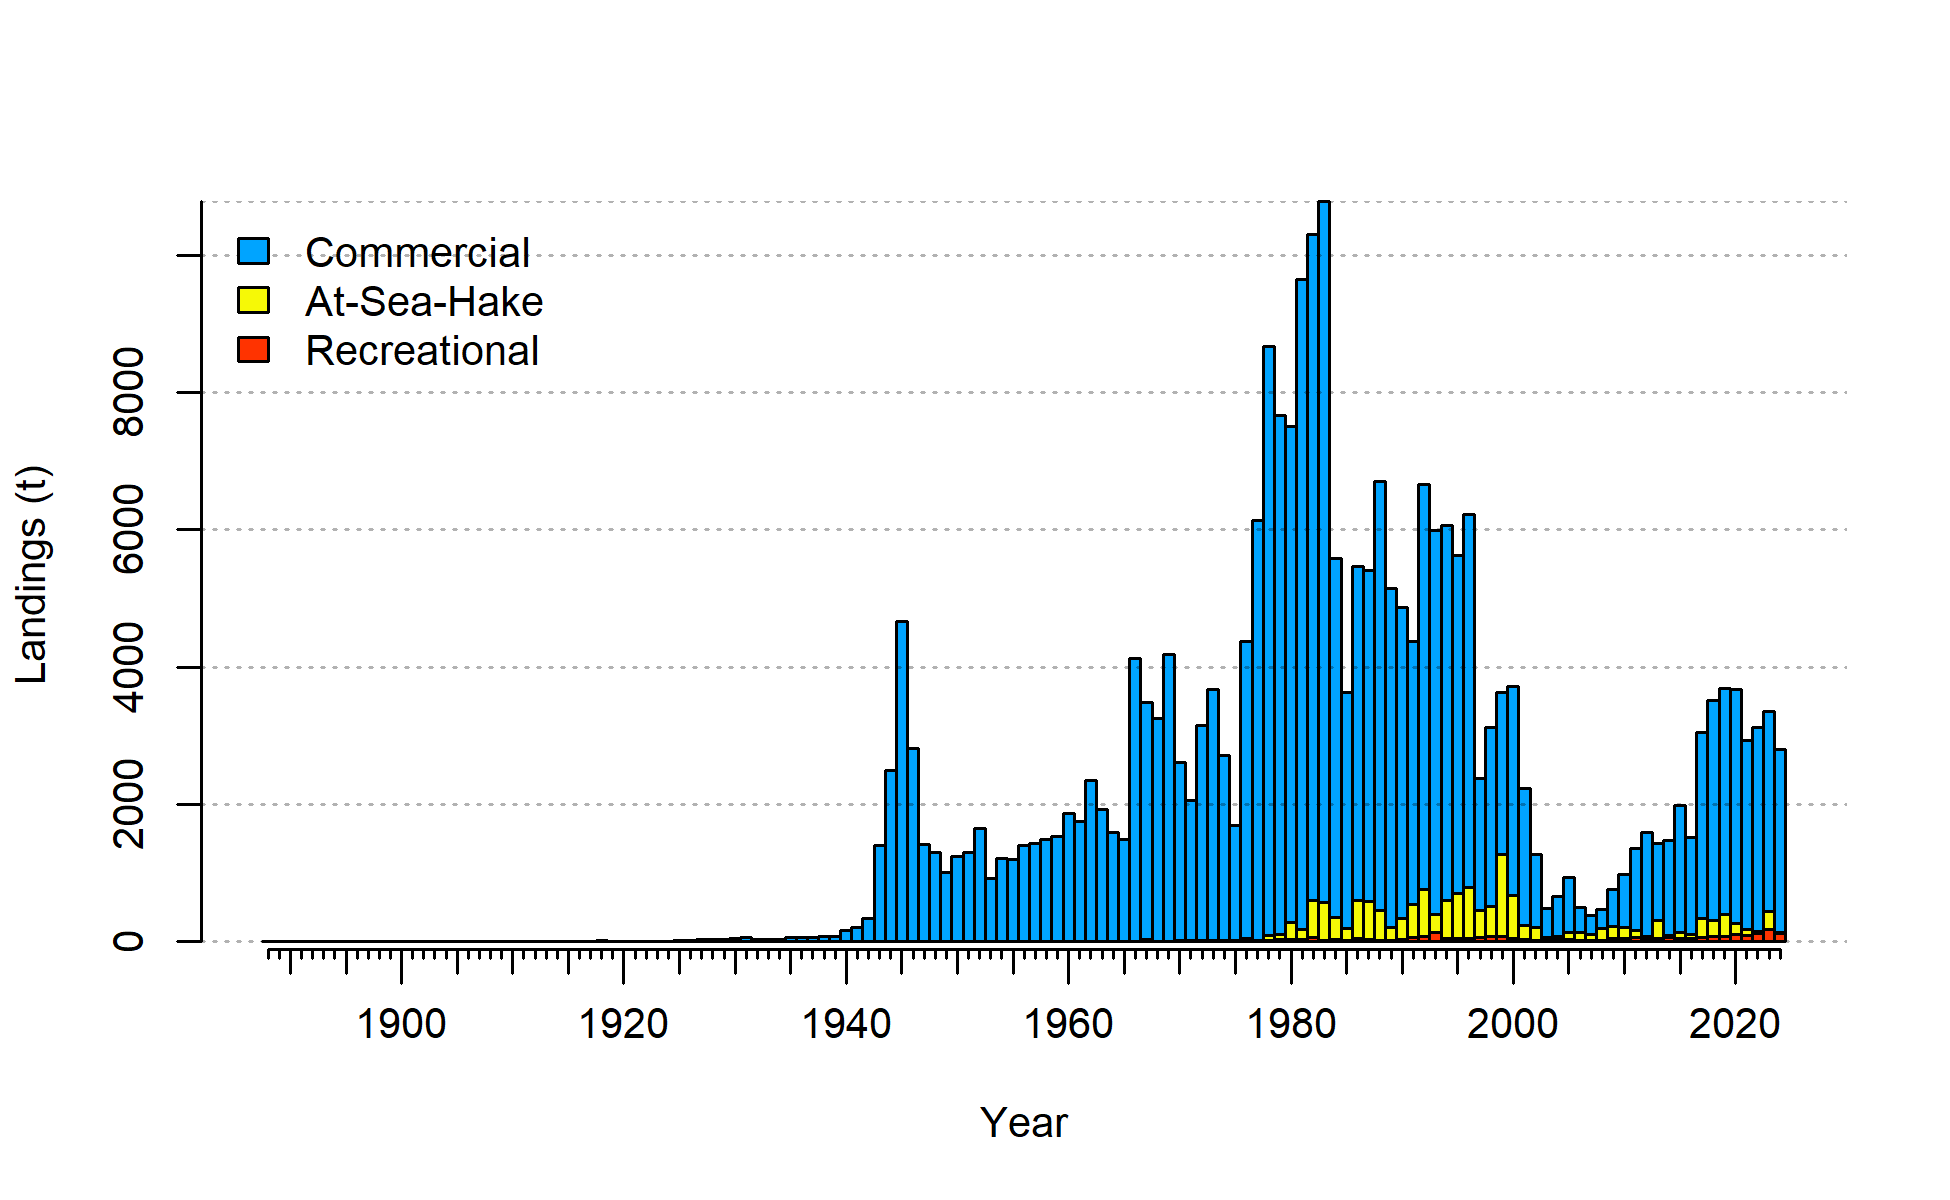
\includegraphics[width=6in,height=\textheight]{r4ss_plots/catch2_landings_stacked.png}

}

\caption{\label{fig-es-catch}Landings by fleet used in the base model
where catches in metric tons by fleet are stacked}

\end{figure}%

\clearpage

\subsubsection{Data and assessment}\label{data-and-assessment}

\subsubsection{Stock biomass and
dynamics}\label{stock-biomass-and-dynamics}

\clearpage 
\begingroup\fontsize{10}{12}\selectfont
\begingroup\fontsize{10}{12}\selectfont

\begin{longtable}[t]{r>{\centering\arraybackslash}p{1.14cm}>{\centering\arraybackslash}p{1.14cm}>{\centering\arraybackslash}p{1.14cm}>{\centering\arraybackslash}p{1.14cm}>{\centering\arraybackslash}p{1.14cm}>{\centering\arraybackslash}p{1.14cm}}
\caption{\label{tab:ssbES}Estimated recent trend in spawning output (trillions of eggs) and the fraction unfished and the 95 percent intervals for the model area.}\\
\toprule
Year & Spawning output (trillions of eggs) & Lower Interval & Upper Interval & Fraction Unfished & Lower Interval & Upper Interval\\
\midrule
\endfirsthead
\caption[]{Estimated recent trend in spawning output (trillions of eggs) and the fraction unfished and the 95 percent intervals for the model area. (\textit{continued)}}\\
\toprule
Year & Spawning output (trillions of eggs) & Lower Interval & Upper Interval & Fraction Unfished & Lower Interval & Upper Interval\\
\midrule
\endhead

\endfoot
\bottomrule
\endlastfoot
2015 & 10.67 & 7.44 & 13.91 & 0.71 & 0.54 & 0.88\\
2016 & 10.74 & 7.49 & 13.99 & 0.71 & 0.54 & 0.88\\
2017 & 10.97 & 7.68 & 14.27 & 0.73 & 0.56 & 0.89\\
2018 & 11.04 & 7.68 & 14.41 & 0.73 & 0.56 & 0.90\\
2019 & 11.07 & 7.62 & 14.51 & 0.73 & 0.56 & 0.90\\
2020 & 11.02 & 7.50 & 14.54 & 0.73 & 0.56 & 0.90\\
2021 & 10.93 & 7.35 & 14.51 & 0.72 & 0.55 & 0.90\\
2022 & 10.89 & 7.27 & 14.50 & 0.72 & 0.55 & 0.90\\
2023 & 10.76 & 7.12 & 14.40 & 0.71 & 0.54 & 0.89\\
2024 & 10.51 & 6.87 & 14.15 & 0.70 & 0.52 & 0.87\\
2025 & 10.27 & 6.65 & 13.89 & 0.68 & 0.51 & 0.85\\*
\end{longtable}
\endgroup{}
\endgroup{}


\begin{figure}

\centering{

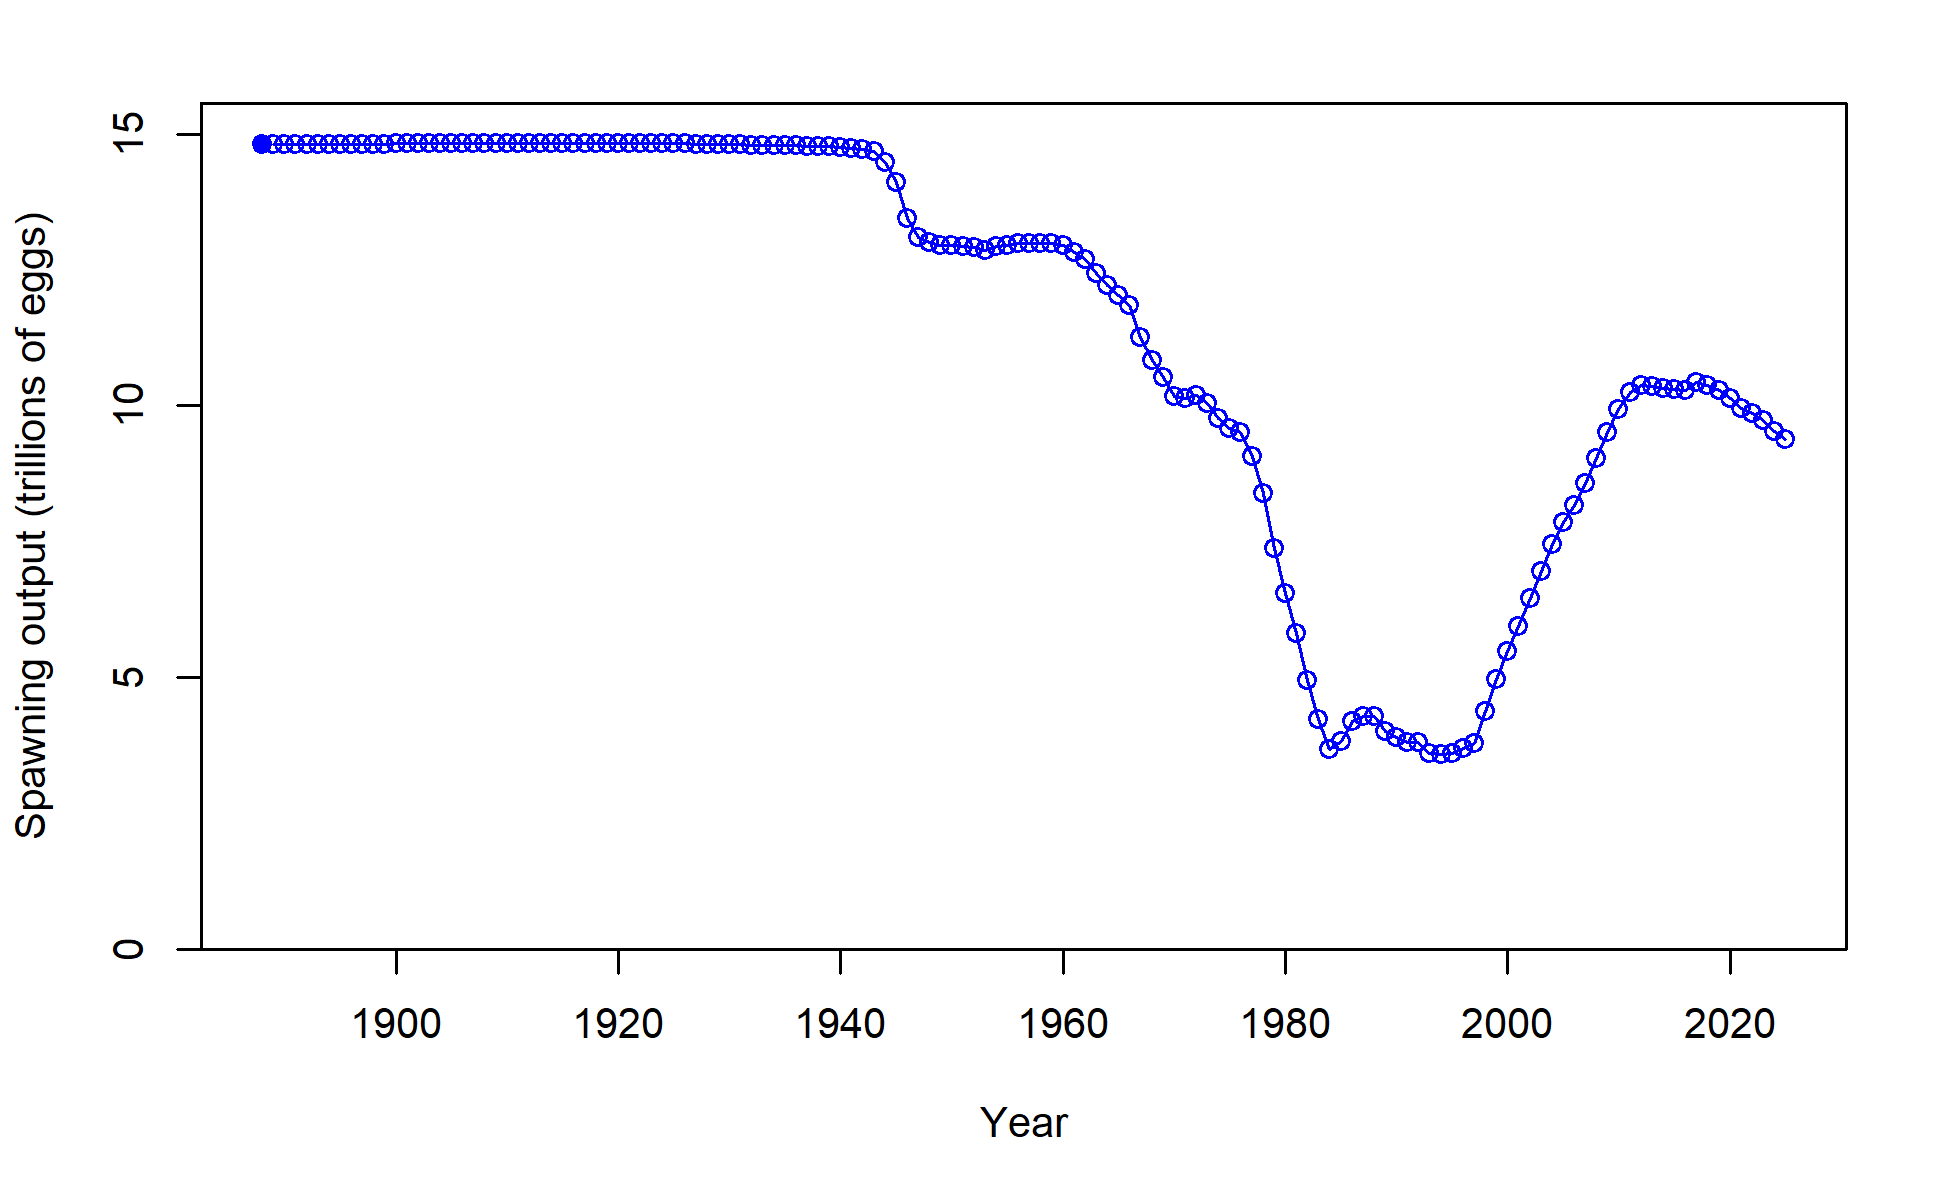
\includegraphics[width=6in,height=\textheight]{r4ss_plots/ts7_Spawning_output.png}

}

\caption{\label{fig-es-ssb}Estimated time series of spawning output for
the base model}

\end{figure}%

\begin{figure}

\centering{

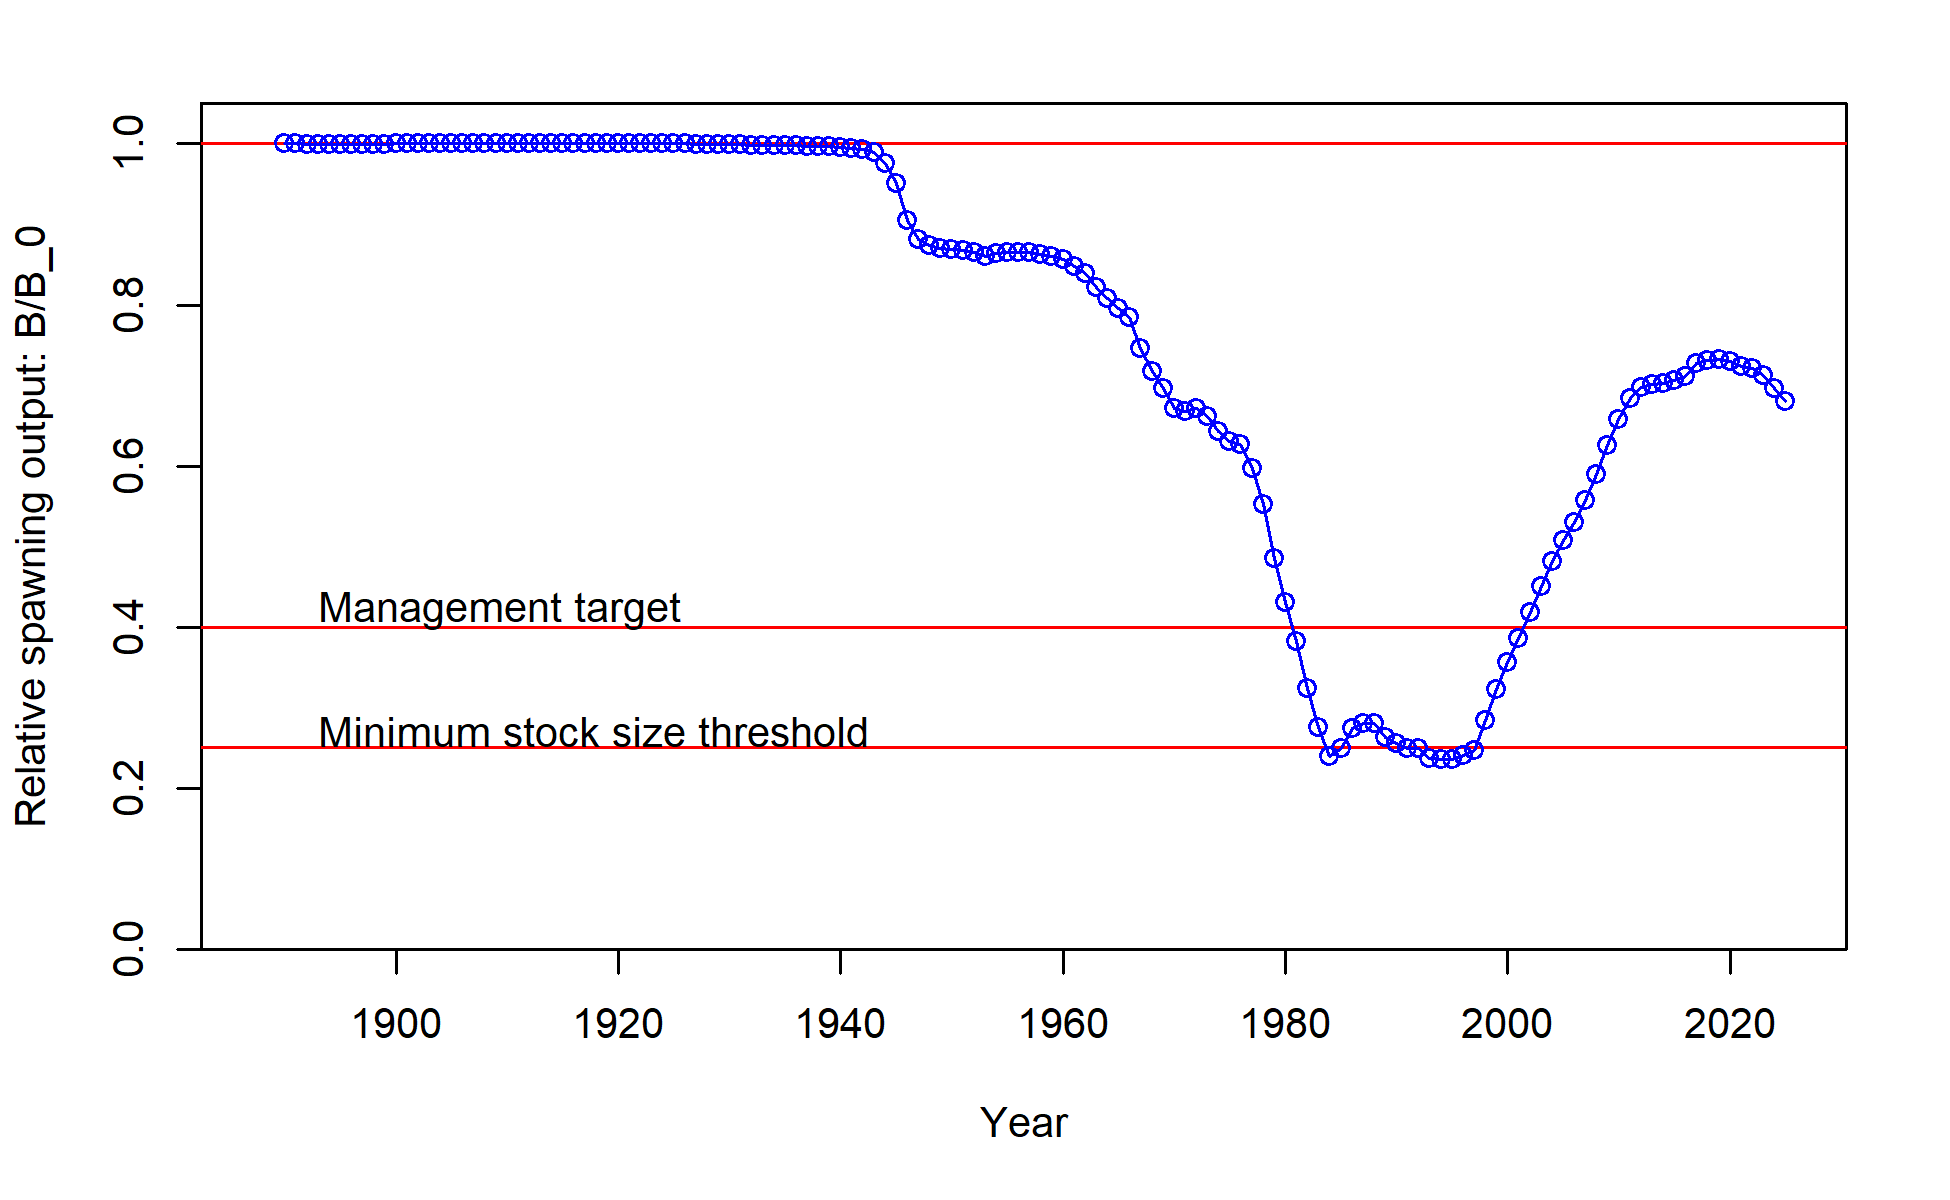
\includegraphics[width=6in,height=\textheight]{r4ss_plots/ts9_Relative_spawning_output.png}

}

\caption{\label{fig-es-frac-unfished}Estimated time series of fraction
of unfished spawning output for the base model}

\end{figure}%

\clearpage

\subsubsection{Recruitment}\label{recruitment}

\begingroup\fontsize{10}{12}\selectfont
\begingroup\fontsize{10}{12}\selectfont

\begin{longtable}[t]{r>{\centering\arraybackslash}p{1.14cm}>{\centering\arraybackslash}p{1.14cm}>{\centering\arraybackslash}p{1.14cm}>{\centering\arraybackslash}p{1.14cm}>{\centering\arraybackslash}p{1.14cm}>{\centering\arraybackslash}p{1.14cm}}
\caption{\label{tab:recrES}Estimated recent trend in recruitment (1,000s) and recruitment deviations and the 95 percent intervals for the model area.}\\
\toprule
Year & Recruitment (1,000s) & Lower Interval & Upper Interval & Recruitment Deviations & Lower Interval & Upper Interval\\
\midrule
\endfirsthead
\caption[]{Estimated recent trend in recruitment (1,000s) and recruitment deviations and the 95 percent intervals for the model area. (\textit{continued)}}\\
\toprule
Year & Recruitment (1,000s) & Lower Interval & Upper Interval & Recruitment Deviations & Lower Interval & Upper Interval\\
\midrule
\endhead

\endfoot
\bottomrule
\endlastfoot
2015 & 24620.3 & 12409.03 & 48848.25 & -0.22 & -0.75 & 0.32\\
2016 & 25269.7 & 12948.93 & 49313.56 & -0.19 & -0.70 & 0.32\\
2017 & 16355.8 & 7873.69 & 33975.45 & -0.64 & -1.24 & -0.04\\
2018 & 14272.3 & 6763.40 & 30117.78 & -0.79 & -1.42 & -0.17\\
2019 & 17825.7 & 8275.36 & 38397.80 & -0.59 & -1.26 & 0.08\\
2020 & 22391.3 & 9531.89 & 52599.27 & -0.38 & -1.17 & 0.41\\
2021 & 29880.7 & 11410.55 & 78248.33 & -0.11 & -1.05 & 0.82\\
2022 & 33758.7 & 12473.12 & 91368.48 & 0.00 & -0.98 & 0.98\\
2023 & 33718.7 & 12454.87 & 91285.63 & 0.00 & -0.98 & 0.98\\
2024 & 33617.6 & 12414.68 & 91032.83 & 0.00 & -0.98 & 0.98\\
2025 & 33514.6 & 12375.79 & 90760.14 & 0.00 & -0.98 & 0.98\\*
\end{longtable}
\endgroup{}
\endgroup{}


\begin{figure}

\centering{

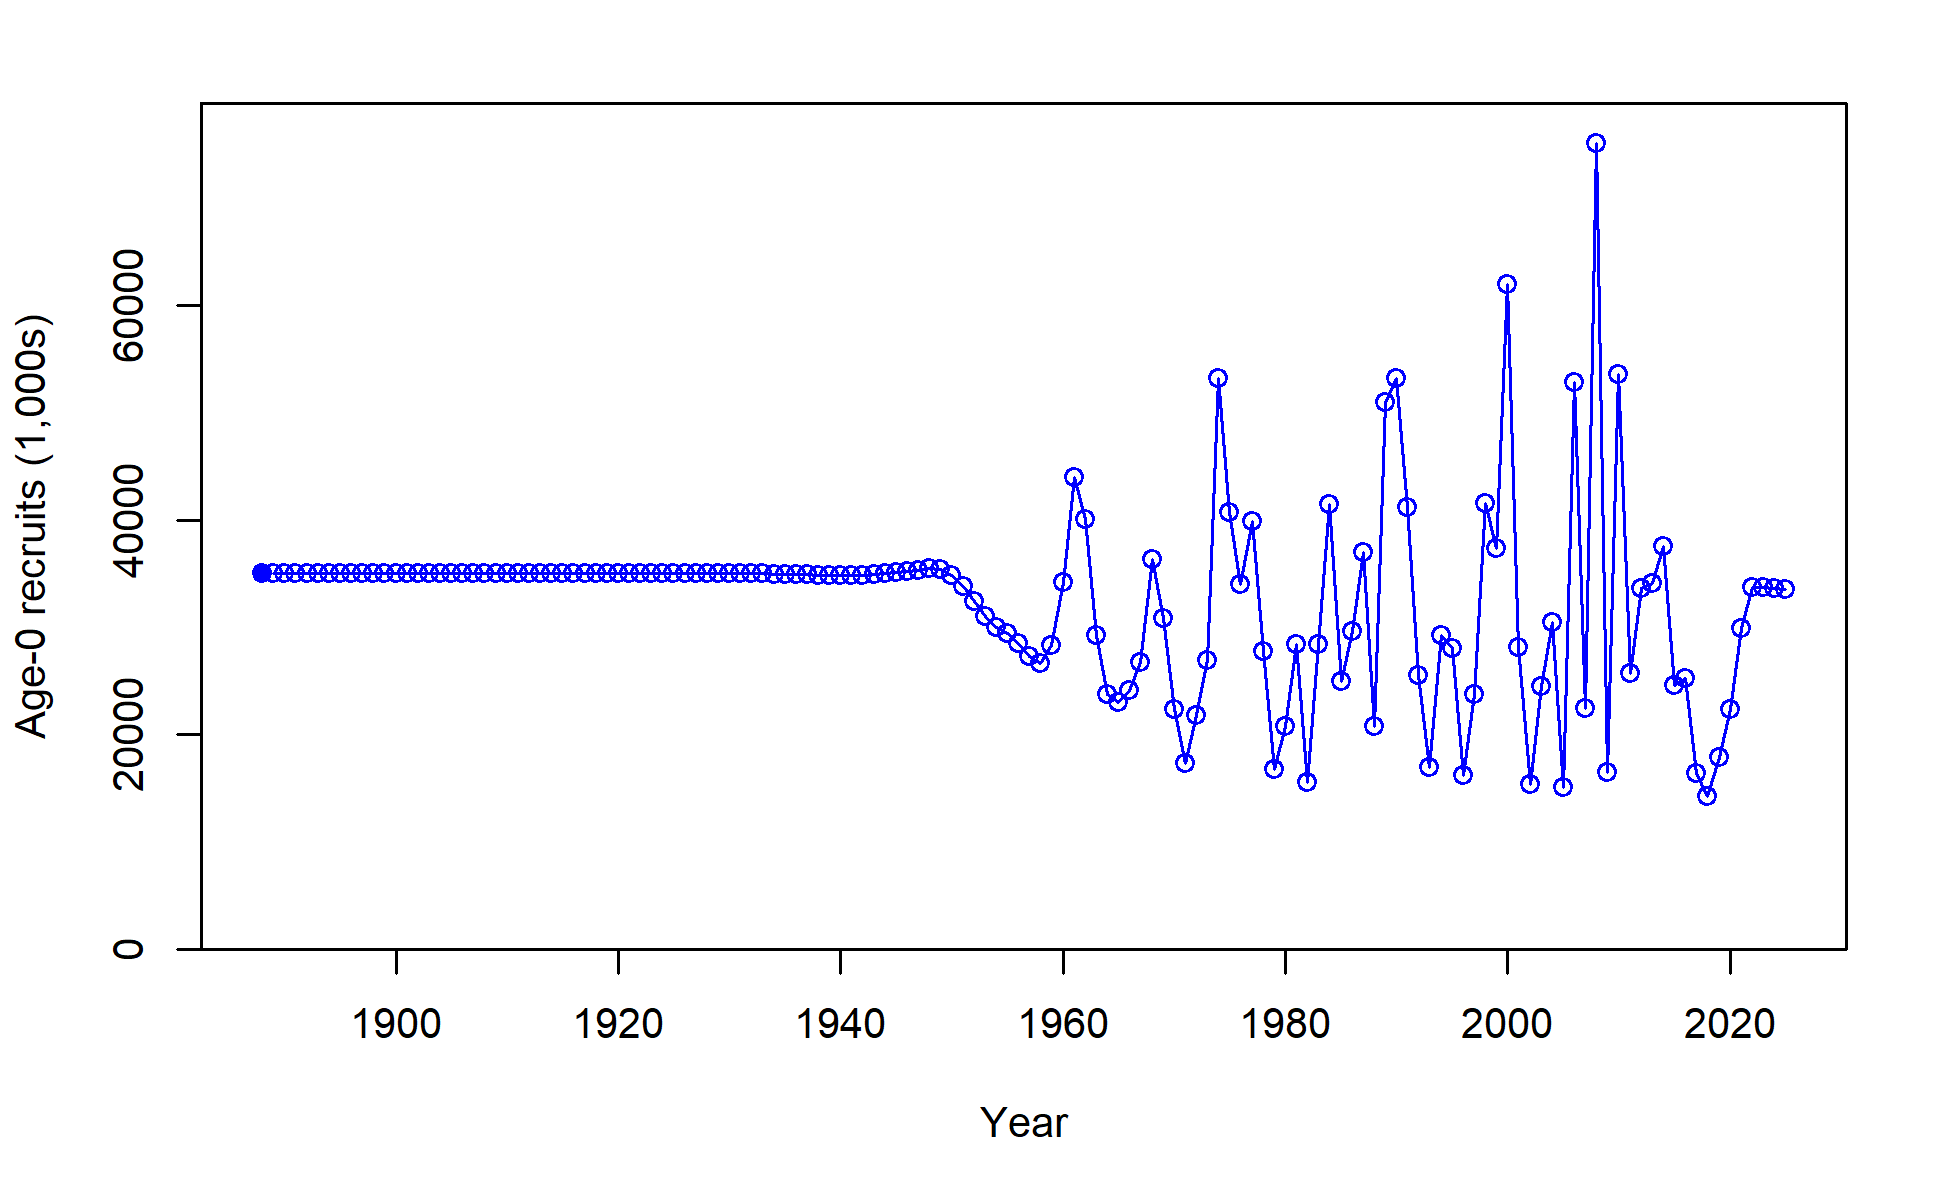
\includegraphics[width=6in,height=\textheight]{r4ss_plots/ts11_Age-0_recruits_(1000s).png}

}

\caption{\label{fig-es-frac-unfished}Estimated time series of age-0
recruits (1000s) for the base model}

\end{figure}%

\begin{figure}

\centering{

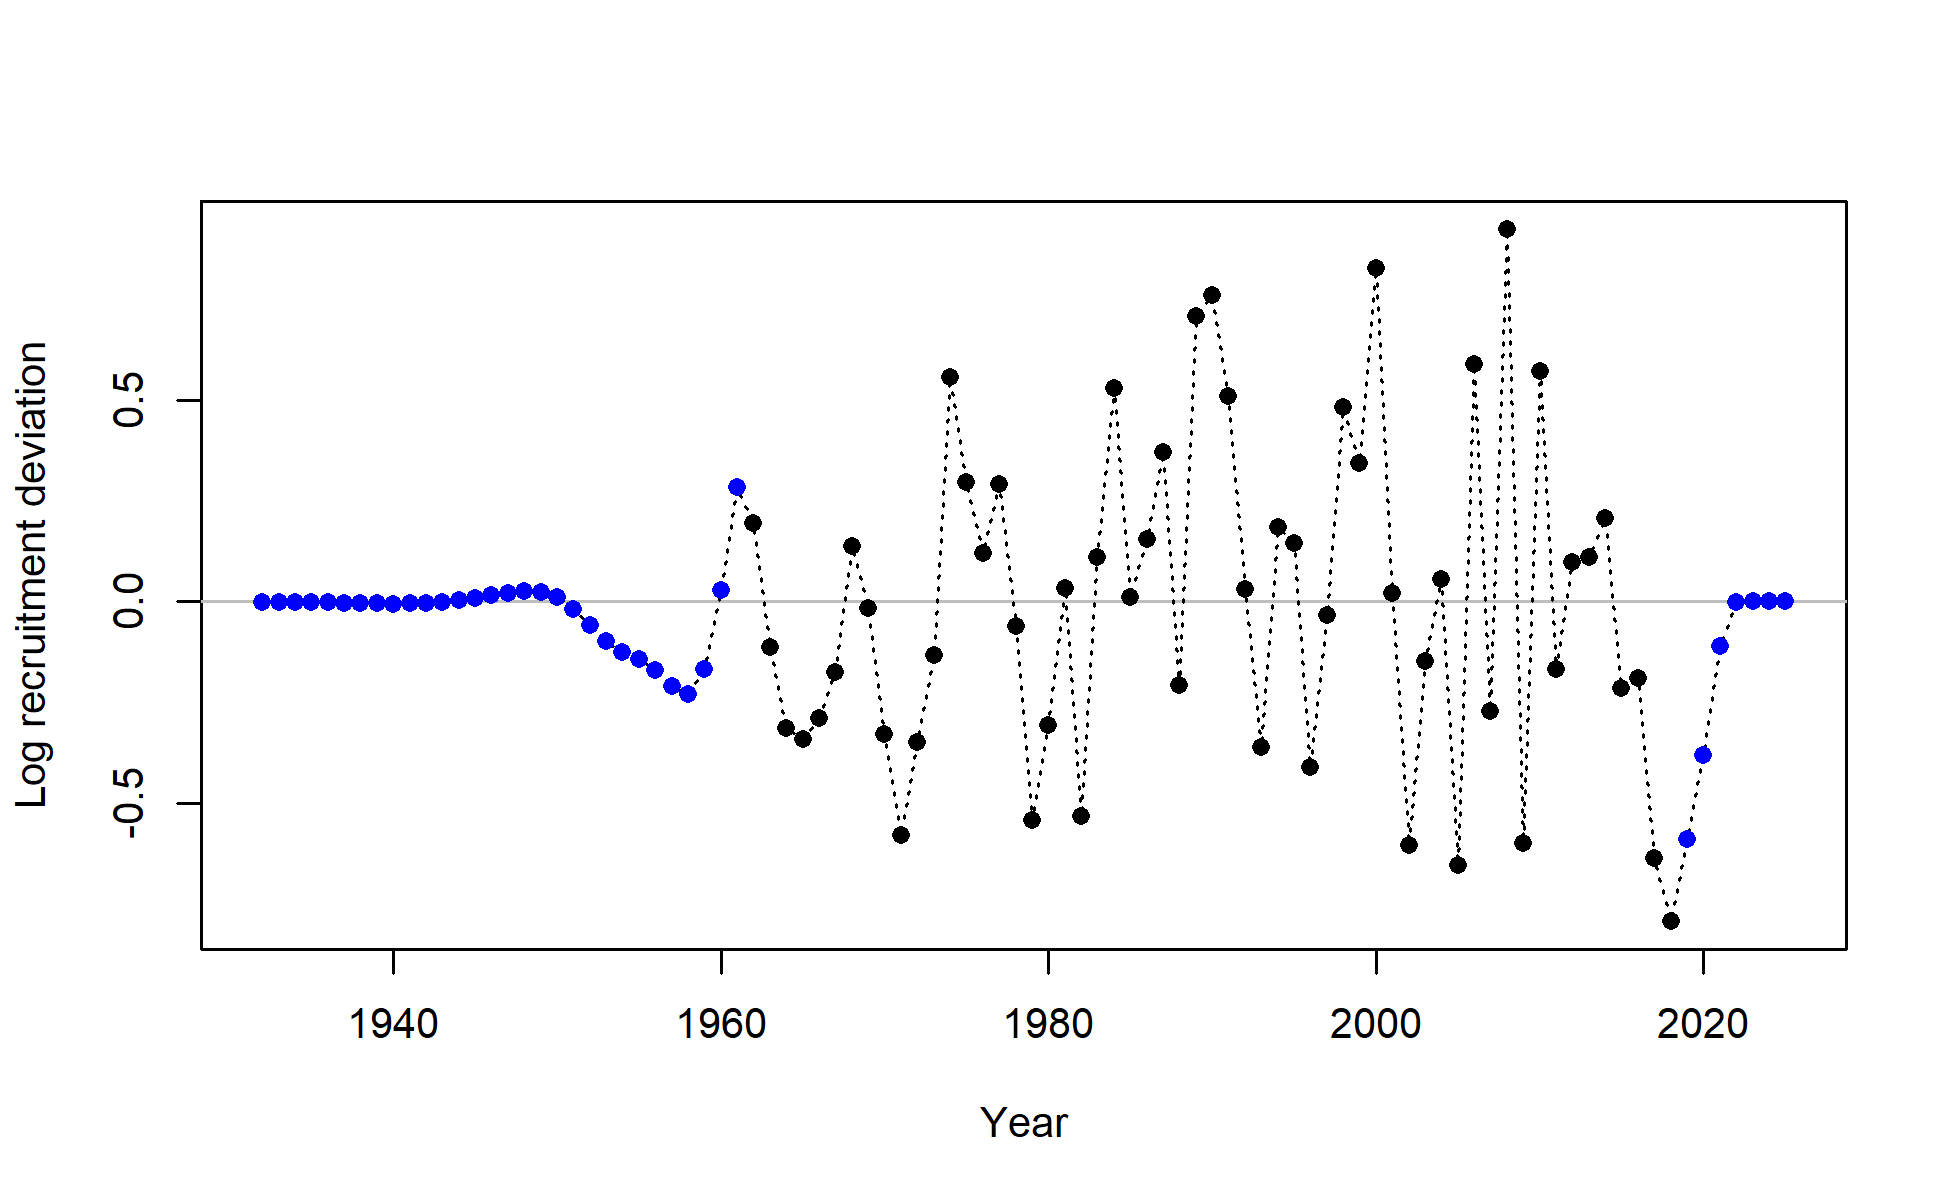
\includegraphics[width=6in,height=\textheight]{r4ss_plots/recdevs1_points.png}

}

\caption{\label{fig-es-rec-devs}Estimated time series of recruitment
deviations for the base model}

\end{figure}%

\clearpage

\subsubsection{Exploitation status}\label{exploitation-status}

\begingroup\fontsize{10}{12}\selectfont
\begingroup\fontsize{10}{12}\selectfont

\begin{longtable}[t]{r>{\centering\arraybackslash}p{1.14cm}>{\centering\arraybackslash}p{1.14cm}>{\centering\arraybackslash}p{1.14cm}>{\centering\arraybackslash}p{1.14cm}>{\centering\arraybackslash}p{1.14cm}>{\centering\arraybackslash}p{1.14cm}}
\caption{\label{tab:exploitES}Estimated recent trend in the (1-SPR)/(1-SPR 50\%) where SPR is the spawning potential ratio, the exploitation rate, and the 95 percent intervals for the model area.}\\
\toprule
Year & (1-SPR)/(1-SPR 50\textbackslash{}\%) & Lower Interval & Upper Interval & Exploitation Rate & Lower Interval & Upper Interval\\
\midrule
\endfirsthead
\caption[]{Estimated recent trend in the (1-SPR)/(1-SPR 50\%) where SPR is the spawning potential ratio, the exploitation rate, and the 95 percent intervals for the model area. (\textit{continued)}}\\
\toprule
Year & (1-SPR)/(1-SPR 50\textbackslash{}\%) & Lower Interval & Upper Interval & Exploitation Rate & Lower Interval & Upper Interval\\
\midrule
\endhead

\endfoot
\bottomrule
\endlastfoot
2015 & 0.46 & 0.31 & 0.60 & 0.02 & 0.01 & 0.02\\
2016 & 0.36 & 0.24 & 0.48 & 0.01 & 0.01 & 0.02\\
2017 & 0.62 & 0.44 & 0.80 & 0.03 & 0.02 & 0.03\\
2018 & 0.68 & 0.49 & 0.87 & 0.03 & 0.02 & 0.04\\
2019 & 0.71 & 0.51 & 0.91 & 0.03 & 0.02 & 0.04\\
2020 & 0.71 & 0.50 & 0.91 & 0.03 & 0.02 & 0.04\\
2021 & 0.60 & 0.42 & 0.79 & 0.03 & 0.02 & 0.04\\
2022 & 0.63 & 0.44 & 0.83 & 0.03 & 0.02 & 0.04\\
2023 & 0.69 & 0.48 & 0.89 & 0.03 & 0.02 & 0.05\\
2024 & 0.61 & 0.42 & 0.80 & 0.03 & 0.02 & 0.04\\*
\end{longtable}
\endgroup{}
\endgroup{}


\begin{figure}

\centering{

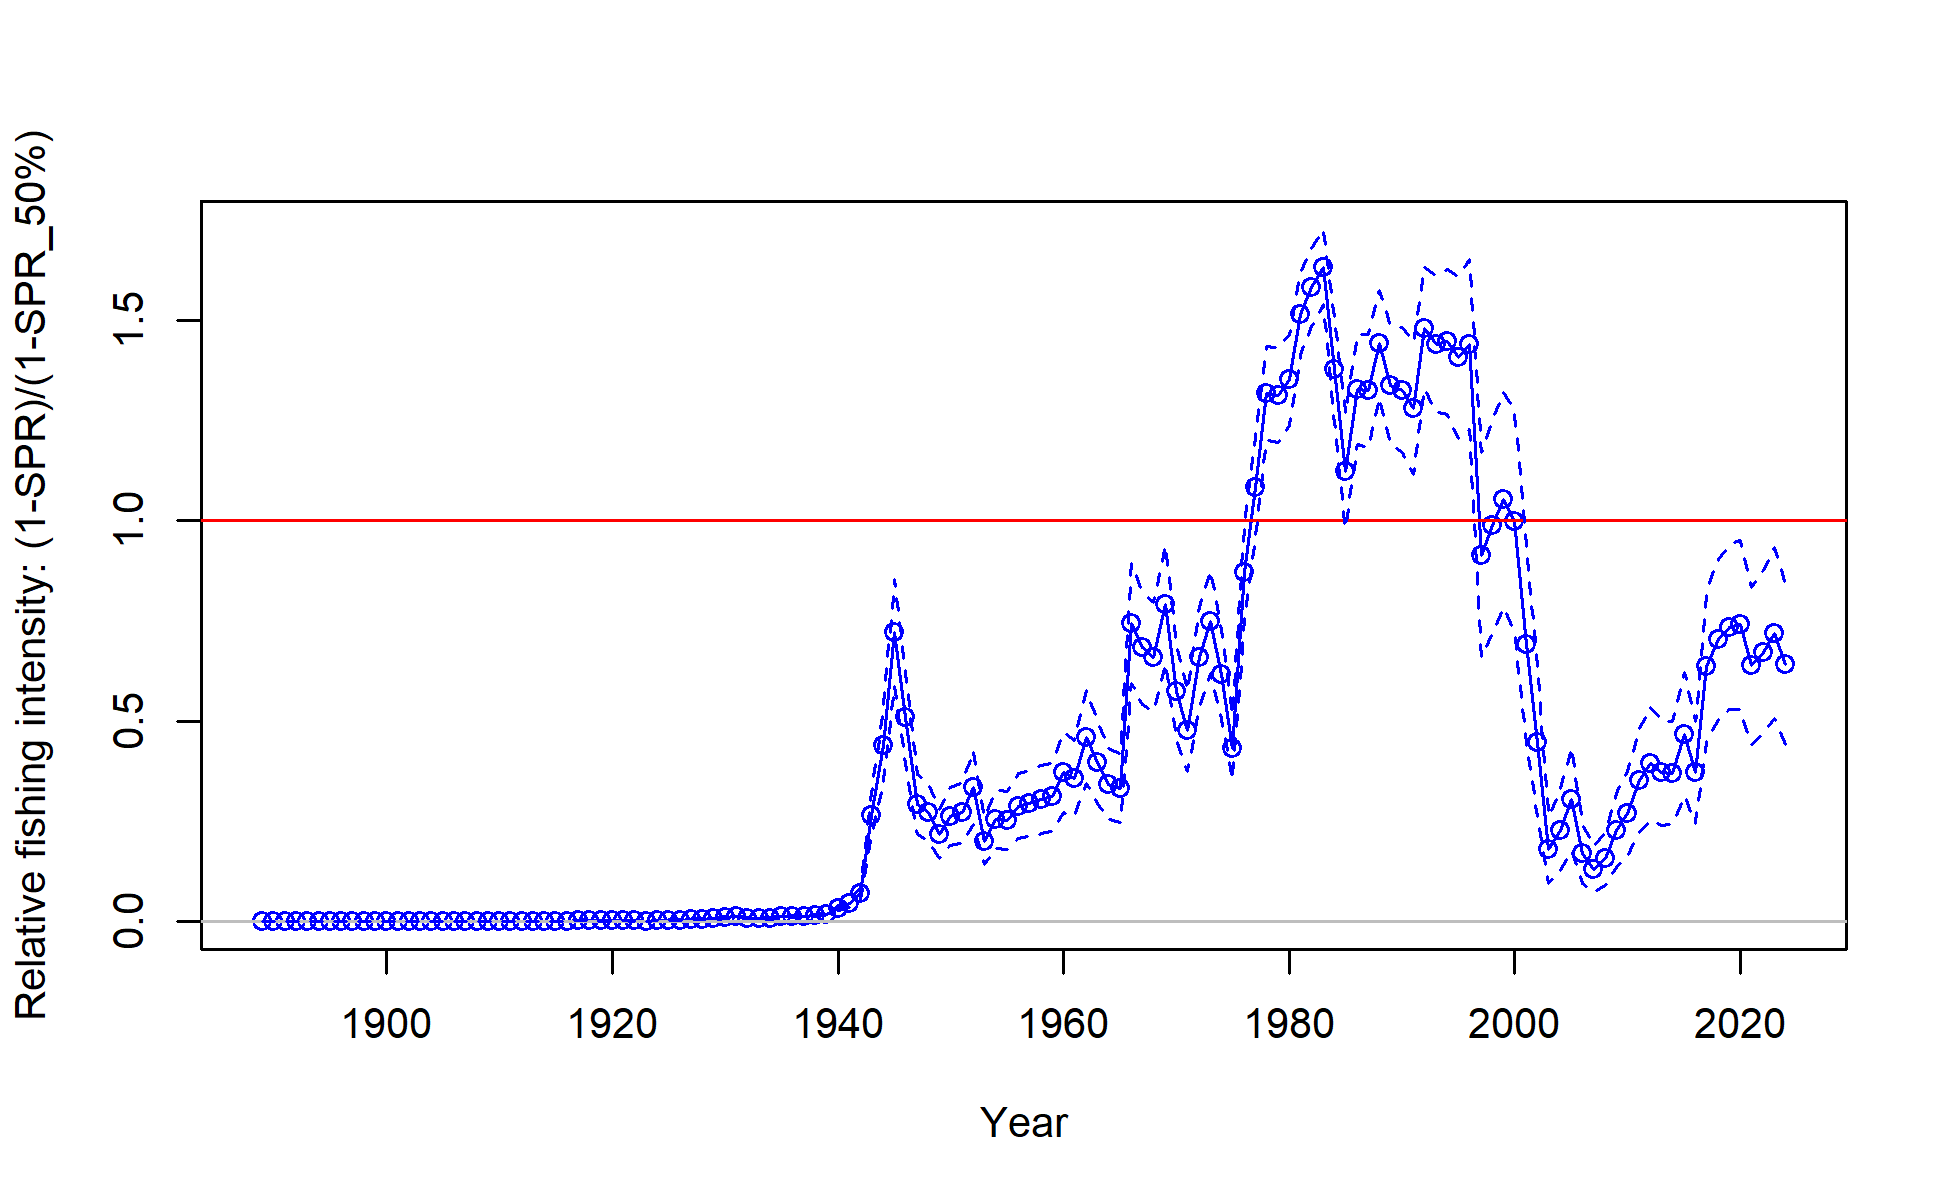
\includegraphics[width=6in,height=\textheight]{r4ss_plots/SPR3_ratiointerval.png}

}

\caption{\label{fig-es-spr}Estimated time series of the fishing
intensity (1 - SPR), where SPR is the spawning potential ratio, with
approximate 95\% asymptotic intervals. The horizontal line at 0.6
corresponds to SPR = 0.4, the management reference point for yellowtail
rockfish. The horizontal line at 1.0 corresponds to SPR = 0 (all
spawning fish removed from the population).}

\end{figure}%

\clearpage

\subsubsection{Ecosystem considerations}\label{ecosystem-considerations}

\subsubsection{Reference points}\label{reference-points}

\clearpage

\begingroup\fontsize{10}{12}\selectfont
\begingroup\fontsize{10}{12}\selectfont

\begin{longtable}[t]{r>{\centering\arraybackslash}p{2cm}>{\centering\arraybackslash}p{2cm}>{\centering\arraybackslash}p{2cm}}
\caption{\label{tab:referenceES}Summary of reference points and management quantities, including estimates of the 95 percent intervals for the model area.}\\
\toprule
Reference Points & Estimate & Lower Interval & Upper Interval\\
\midrule
\endfirsthead
\caption[]{Summary of reference points and management quantities, including estimates of the 95 percent intervals for the model area. (\textit{continued)}}\\
\toprule
Reference Points & Estimate & Lower Interval & Upper Interval\\
\midrule
\endhead

\endfoot
\bottomrule
\endlastfoot
Unfished Spawning output (trillions of eggs) & 15.10 & 13.01 & 17.19\\
Unfished Age 4+ Biomass (mt) & 134833.00 & 112503.13 & 157162.87\\
Unfished Recruitment (R0) & 35014.50 & 21427.32 & 48601.68\\
2025 Spawning output (trillions of eggs) & 10.27 & 6.65 & 13.89\\
2025 Fraction Unfished & 0.68 & 0.51 & 0.85\\
Reference Points Based SO40\textbackslash{}\% & NA & NA & NA\\
Proxy Spawning output (trillions of eggs) SO40\textbackslash{}\% & 6.04 & 5.20 & 6.88\\
SPR Resulting in SO40\textbackslash{}\% & 0.46 & 0.46 & 0.46\\
Exploitation Rate Resulting in SO40\textbackslash{}\% & 0.06 & 0.05 & 0.06\\
Yield with SPR Based On SO40\textbackslash{}\% (mt) & 4487.15 & 3533.09 & 5441.21\\
Reference Points Based on SPR Proxy for MSY & NA & NA & NA\\
Proxy Spawning output (trillions of eggs) (SPR50) & 6.73 & 5.80 & 7.66\\
SPR50 & 0.50 & NA & NA\\
Exploitation Rate Corresponding to SPR50 & 0.05 & 0.05 & 0.05\\
Yield with SPR50 at SO SPR (mt) & 4235.93 & 3340.87 & 5130.99\\
Reference Points Based on Estimated MSY Values & NA & NA & NA\\
Spawning output (trillions of eggs) at MSY (SO MSY) & 3.56 & 3.04 & 4.07\\
SPR MSY & 0.31 & 0.31 & 0.32\\
Exploitation Rate Corresponding to SPR MSY & 0.09 & 0.08 & 0.09\\
MSY (mt) & 4994.84 & 3902.57 & 6087.11\\*
\end{longtable}
\endgroup{}
\endgroup{}


\begin{figure}

\centering{

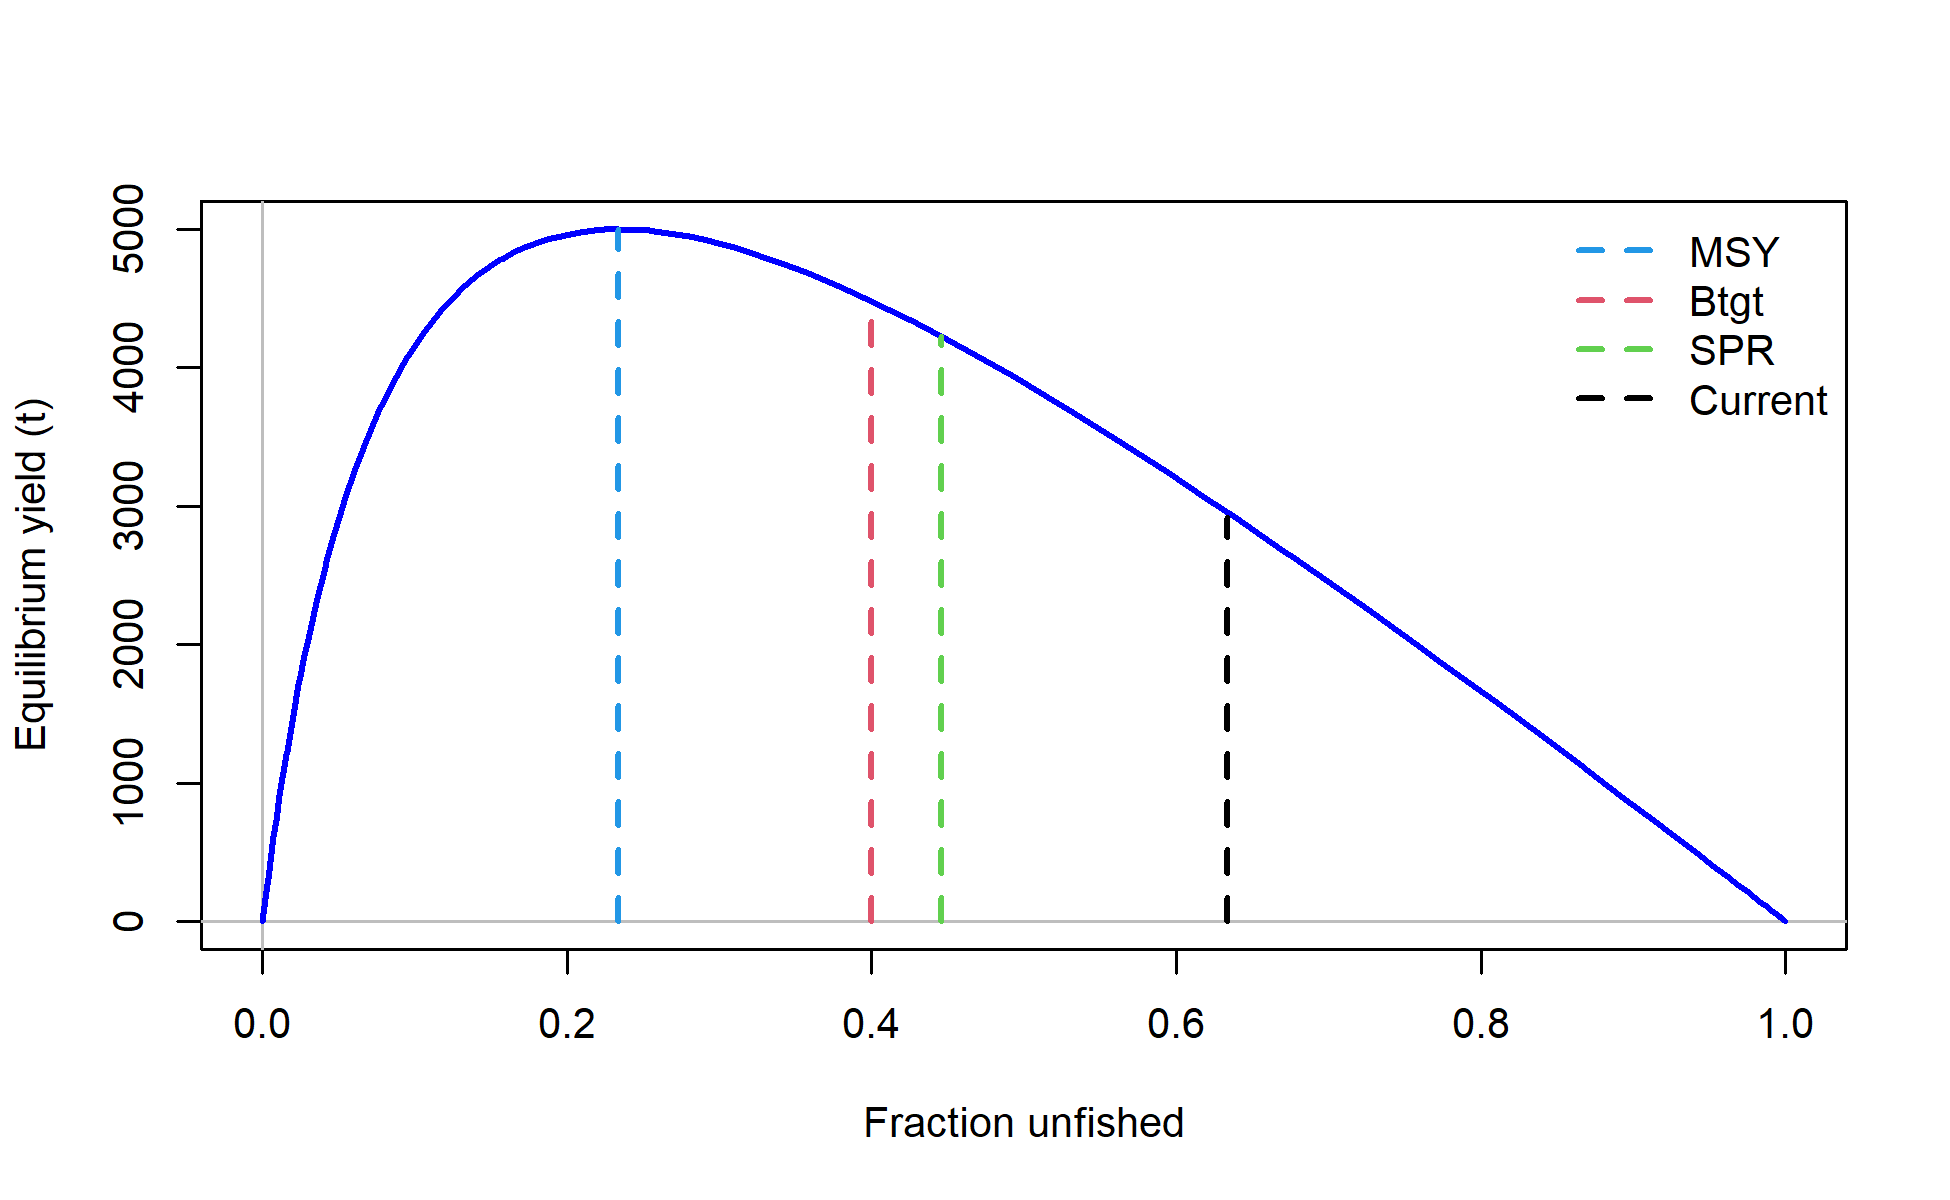
\includegraphics[width=6in,height=\textheight]{r4ss_plots/yield2_yield_curve_with_refpoints.png}

}

\caption{\label{fig-es-yield}Equilibrium yield curve for the base case
model.}

\end{figure}%

\clearpage

\subsubsection{Management performance}\label{management-performance}

\subsubsection{Unresolved problems and major
uncertainties}\label{unresolved-problems-and-major-uncertainties}

\subsubsection{Decision table and
projections}\label{decision-table-and-projections}

\clearpage

\clearpage

\subsubsection{Scientific uncertainty}\label{scientific-uncertainty}

\subsubsection{Research and data needs}\label{research-and-data-needs}

\newpage{}

\section{Introduction}\label{introduction}

Yellowtail Rockfish, \emph{Sebastes flavidus}, occur off the West Coast
of the United States from Baja California to the Aleutian Islands.
Yellowtail is a major commercial species, captured mostly in trawls from
Central California to British Columbia (\citeproc{ref-Love2011}{Love
2011}). Because it is an aggregating, midwater species it is usually
caught in the commercial midwater trawl fishery. In California there is
a large recreational fishery as well. The center of Yellowtail Rockfish
abundance is from southern Oregon through British Columbia
(\citeproc{ref-Fraidenburg1980}{Fraidenburg 1980}). Yellowtail Rockfish
are colloquially known as ``greenies'', although \emph{flavidus} is
Latin for ``yellow'' (\citeproc{ref-Love2011}{Love 2011}). We briefly
summarize Yellowtail Rockfish life history, fisheries, assessment and
management here, but in-depth, extensive background information on
Yellowtail Rockfish and other managed species is available at
(\citeproc{ref-PFMC2016}{Council 2016}).

A number of studies correlate environmental conditions to pelagic
juvenile abundance and juvenile recruitment of rockfishes, including
Yellowtail Rockfish. Year-class strength is particularly impacted during
the early larval phase, and annual pelagic juvenile abundance is
correlated with physical conditions, especially upwelling strength along
the coast (e.g., (\citeproc{ref-Field2005}{Field and Ralston 2005}),
(\citeproc{ref-Laidig2007}{Laidig, Chess, and Howard 2007}),
(\citeproc{ref-Laidig2010}{Laidig 2010}),
(\citeproc{ref-Ralston2013}{Ralston and Stewart 2013})).

A recent genetic study (\citeproc{ref-Hess2011}{Hess, Vetter, and Moran
2011}) indicates that there are in fact two stocks of Yellowtail
Rockfish, with a genetic cline at Cape Mendocino, California, roughly
\(40^\circ 10^\prime\) North Latitude. This study of 1013 fish from 21
sites along the West Coast from Mexico through Alaska examined two
datasets, one of mitochondrial DNA, and one of nuclear DNA
microsattelite loci. Findings in both datasets agreed, and also concur
with the findings of Field and Ralston (\citeproc{ref-Field2005}{Field
and Ralston 2005}) who looked at differences in recruitment trends
related to physical forcing and coherence along the coast, and found the
greatest differences among the U.S. and Canadian stocks to be defined by
Cape Mendocino. Neither the genetic study nor the oceanographic studies
definitively identify mechanisms of stock isolation, however they
suggest that a combination of physical forcing due to offshore advection
and differences in available habitat across Cape Mendocino may together
account for the differences observed.

The species has never had a full length and age integrated assessment
south of Cape Mendocino, mainly due to a lack of fishery-independent
data; this assessment represents an initial attempt to do so.

A map showing the scope of the assessment and depicting boundaries for
fisheries or data collection strata is provided in Figure
\ref{fig:assess_region_map}.

\subsection{Life History}\label{life-history}

\subsection{Ecosystem considerations}\label{ecosystem-considerations-1}

\subsection{Fishery description}\label{fishery-description}

\subsection{Management History}\label{management-history}

\subsection{Management performance}\label{management-performance-1}

\subsection{Fisheries off Canada and
Alaska}\label{fisheries-off-canada-and-alaska}

\newpage{}

\section{Data}\label{data}

\subsection{Fishery-dependent data}\label{fishery-dependent-data}

\subsubsection{Landings}\label{landings}

\subsubsection{Discards}\label{discards}

\subsubsection{Biological data}\label{biological-data}

\subsubsection{Abundance indices}\label{abundance-indices}

\paragraph{Oregon ORBS Dockside Index (2001 -
2024)}\label{oregon-orbs-dockside-index-2001---2024}

Trip-level catch-per-unit-effort data from ORBS dockside sampling was
obtained from ODFW. To mitigate the confounding of hourly effort
associated with these trips with travel, the travel time was subtracted
from the hours fished. Travel time was stratified by boat type (charter
and private) and was calculated as boat type-specific speeds (13 mph for
charter boat trips and 18 mph for private boat trips) multiplied by
twice the distance between the port of origin and the reef that was
fished. CPUE, expressed in terms of fish per angler-hour, was calculated
by multiplying the number of anglers and the adjusted travel time. The
database contains information on catch by species (number of retained
fish), effort (angler hours), sample location (port where data were
collected), date, bag limits and other relevant regulations, boat type
(charter or private), and trip type (e.g., bottom associated fish).

The unfiltered data set contained 456,172 trips from 2001 - 2024.
Multiple standardized filters are applied to ORBS trip-level data to
remove outliers and data unsuitable for an index. These filters include
trips with incorrect interview times, which impact calculation of
effort, unreasonably long or short trips, and retaining only bottomfish
target trips. Further filters were utilized for fishing closures
(i.e.~temporal or spatial closures) and catches exceeding bag limits,
which would presumably impact catch rates. Trips from several ports with
extremely small sample sizes (\textless1\% of total trips) were also
excluded and finally, trips that met criteria for irrational effort
reporting (i.e., implausible values) or extreme catch rates were
excluded as well. The final dataset included 137,502 trips (TABLE
``percent\_pos.csv'').

Covariates evaluated included year, month, port, the open depths to
fishing (all depths or inside 20/30/40fm), boat type and the daily bag
limit for Yellowtail Rockfish. Preliminary model explorations indicated
that the daily bag limit covariate could not be combined with the open
depth of the fishery due to changes in recreational fishing regulations
over time. Prior to 2017, Yellowtail Rockfish were included in the
general marine bag limit. However, in 2017, Yellowtail Rockfish were
also included in a specialized longleader recreational bag limit where
participants were required to be outside of 40fm. As a result, the bag
limits were binned into a binary covariate for low (5 -- 8 fish) and
high (10 -- 15fish) bag limits during the 2001 -- 2024 time period.
Negative binomial models were fit in sdmTMB (Version 0.6.0) to the
trip-level data (catch with a log offset for adjusted angler hours).
Tweedie distributions were also explored for selected models but
generally did not improve model diagnostics. The final model selected
includes year, month, port, open fishery depths, longleader trip and
binned target bag limit covariates, which was the best fit model by AIC
in this series (TABLE ``model\_selection.csv''). Acceptable diagnostics
for the model were achieved (FIGURE -- qqplot) and the negative binomial
distribution was preferred over the tweedie. The index of abundance are
shown in Figure/Table XXXX.

\subsection{Fishery-independent data}\label{fishery-independent-data}

\subsubsection{Abundance Indices}\label{abundance-indices-1}

\paragraph{SMURF YOY Index}\label{smurf-yoy-index}

ODFW and Oregon State University (OSU) have collaborated on young of the
year (YOY) fish and environmental monitoring in and around Oregon Marine
Reserves (MR) using SMURF devices, standardized sampling units that
collect newly-settled juvenile fishes. Data were provided for two
regions on the Oregon coast, near the Otter Rock MR (central) and the
Redfish Rocks MR (southern) with a site inside of the reserve and a
comparison site outside of the reserve from 2011 to the present. These
are monitored regularly (approximately every 2 weeks) during the
settlement season (April - September) and YOY are collected for genetic
identification and measured. Settlement rate of YOY Yellowtail Rockfish
was provided by OSU for each site within each region. Paired temperature
at depth data was provided by ODFW MR Ecological Monitoring team for
this assessment. Daily mean temperature data was provided for three
depth strata (1m, 7.5m, and 15m) for each site within each region.

Oceanographic sampling by the ODFW MR Ecological Monitoring team has not
been able to be done simultaneously in both reserves at each mooring
site at all depths due to a lack of equipment. However, for time periods
when there was matched data, temperature was highly correlated across
depths (Pearson's correlation coefficient \textgreater{} 0.90) and
between sites within each region (Pearson's correlation coefficients
\textgreater0.98). In order to calculate an index of daily water column
temperature that was continuous enough to be combined with settlement
rate data, temperature data was standardized within year and depth. For
periods with multiple observations, the mean was taken in order to
generate a single continuous temperature time series. Mean SMURF
deployment lasted 15.5 days. In order to summarize temperature in an
ecologically meaningful way relative to the SMURF sampling design, a
16-day rolling mean of temperature and cumulative degree days over
16-day periods were calculated. These data were matched with settlement
rate data such that the mean temperature or the cumulative degree days
during the 16-day period that the SMURF was deployed was used.

Covariates evaluated for were year, month, region (Redfish Rocks or
Otter Rock), temperature, and site (within marine reserve or nearby
comparison site). Preliminary model runs indicated a consistent lack of
convergence and additional filters were applied to address this,
including limiting the data to 2014 - 2024 and to the peak months of
settlement for yellowtail (May - July). Month was not included in models
that included temperature as both covariates were used to describe
seasonal variation in settlement rate. Site was not a significant
covariate in this model but this was not unexpected, as the presence of
a reserve would not be anticipated to impact juvenile settlement rates.
Models were fit to the settlement rate data (YOY fish per day) using
sdmTMB R package (Version 0.6.0). Both negative binomial and tweedie
distributions were evaluated. The model that was selected based on fit
(TABLE X) and expert opinion from OSU and ODFW staff. The final model
contained year, region, and temperature summarized as cumulative degree
days 16-days prior to SMURF recovery using a negative binomial
distribution. Acceptable model convergence and other diagnostic criteria
for the final index were achieved (FIGURE - qqplot). The index of YOY
abundance and associated standard errors are shown in Figure/Table Y.

\subsection{Biological Parameters}\label{biological-parameters}

\subsubsection{Natural Mortality}\label{natural-mortality}

\subsubsection{Weight-at-length}\label{weight-at-length}

\subsubsection{Maturity}\label{maturity}

We used a total of 292 individual histological samples of aged female
yellowtail rockfish to estimate maturity for the assessment. These
samples were all collected north of 40.167; this latitude filter
excluded 5 additional samples collected in the south, but the inclusion
or exclusion of these samples did not change our results. The 292
samples were collected over the period 2016---2023, though more samples
were collected earlier in these years (n = 111 in 2016, 52 in 2017, 31
in 2018, 17 in 2021, 9 in 2022, 13 in 2023). Previous assessments of
yellowtail estimated length-based maturity (L50 = 42.49cm in 2017
assessment); however, we switched to an age based model for the current
assessment. For many species, energy is reallocated toward maturation
from growth, and as a result growth rates slow during the juvenile to
adult transition period. Thus, length at 50\% maturity will represent a
range of ages, providing a less accurate understanding of the spawning
population. We treated maturity as a binomial response, and considered a
variety of models with temporal and spatial covariates, using a logit
link and generalized linear mixed model framework, implemented the R
package sdmTMB (\citeproc{ref-Anderson:2024:SRP}{Anderson et al. 2024}).
Briefly, we considered models that included (1) temporal year effects
(either estimated as a random walk intercept, or smooth term), (2)
spatial random fields (using a mesh cutoff distance of 50km), and (3)
spatially varying coefficients of age, following the model adopted by
Grandin et al. (\citeproc{ref-grandin_status_2024}{2024}). Models that
converged were compared by examining QQ plots, AUC metrics, and AIC
scores. Likely because of the uneven temporal distribution of sampling,
and general sparsity, we did not find support for including temporal or
spatial effects, and decided on the simpler null model (equivalent to a
logistic regression). For the age-based model, we estimated an intercept
of -6.70 (SE = 0.99) and slope of 0.67 (SE = 0.10), equivalent to an A50
of 10.0 years. For a more direct comparison to the previous assessment,
we used these same 292 samples to fit an equivalent length -- based
model, which resulted in an estimated L50 = 42.5 cm.

\subsubsection{Fecundity}\label{fecundity}

\subsection{Environmental and ecosystem
data}\label{environmental-and-ecosystem-data}

\subsubsection{Oceanographic Index}\label{oceanographic-index}

Over the past several years, progress has been made in understanding how
oceanographic conditions drive recruitment of groundfish species in the
California Current Ecosystem across lifestages including petrale sole,
sablefish and hake. Recent increases in capacity supported by the
Climate, Ecosystem, and Fisheries Initiative provided the ability to
build on these previous lines of research and examine the relationship
between northern Yellowtail rockfish recruitment and oceanographic
drivers based on model output from Global Ocean Physics Reanalysis
(GLORYS) from \href{https://marine.copernicus.eu/}{Copernicus Marine
Environment Monitoring Service} (CMEMS) and Regional Ocean Modeling
System (ROMS) model for the California Current Ecosystem (Neveu et
al.~2016). The results suggest that GLORYS and ROMS output may allow for
better model precision and near-term forecasting. This approach builds
on previous research (Tolimieri et al.~2020, Haltuch et al.~2020,
Vestfals et al.~2023) and assessments (Taylor et al.~2023, Johnson et
al.~2023) by applying similar techniques to establish oceanographic
relationships and develop an oceanographic index based on a conceptual
life history model for yellowtail rockfish (Darby et al.~in prep).
GLORYS also provides a temporally robust time series and is not
susceptible to discontinuities identified in the 2023 petrale sole
assessment. Appendix A of this report describes the most recent efforts
in developing a new environmental index of northern Yellowtail
recruitment based on GLORYS products. The final selected model included
the date of spring transition from the Coastal Upwelling Transport
Index, degree days (represent temperature exposure) during egg
fertilization and development, long-shore transport during the pelagic
juvenile lifestage, and El Nino conditions during the pelagic juvenile
lifestage. The oceanographic model was fit using the recruitment
deviations (1994 - 2019) from the base model and used to predict log
recruitment deviations 5 years ahead, 2020 - 2024, using oceanographic
conditions.

\newpage{}

\section{Assessment model}\label{assessment-model}

\subsection{History of modeling
approaches}\label{history-of-modeling-approaches}

\subsection{Response to most recent STAR panel and SSC
recommendations}\label{response-to-most-recent-star-panel-and-ssc-recommendations}

\subsection{Model Structure and
Assumptions}\label{model-structure-and-assumptions}

\subsubsection{Model Changes from the Last
Assessment}\label{model-changes-from-the-last-assessment}

\subsubsection{Modeling Platform and
Structure}\label{modeling-platform-and-structure}

\subsubsection{Model Parameters}\label{model-parameters}

\subsubsection{Key Assumptions and Structural
Choices}\label{key-assumptions-and-structural-choices}

\newpage{}

\subsection{Base Model Results}\label{base-model-results}

\subsubsection{Parameter Estimates}\label{parameter-estimates}

\subsubsection{Fits to the Data}\label{fits-to-the-data}

\subsubsection{Population Trajectory}\label{population-trajectory}

\newpage{}

\subsection{Model Diagnostics}\label{model-diagnostics}

\subsubsection{Convergence}\label{convergence}

\subsubsection{Sensitivity Analyses}\label{sensitivity-analyses}

\subsubsection{Retrospective Analysis}\label{retrospective-analysis}

\subsubsection{Likelihood Profiles}\label{likelihood-profiles}

\subsection{Unresolved Problems and Major
Uncertainties}\label{unresolved-problems-and-major-uncertainties-1}

\newpage{}

\section{Management}\label{management}

\subsection{Reference Points}\label{reference-points-1}

\subsection{Harvest Projections and Decision
Tables}\label{harvest-projections-and-decision-tables}

\subsection{Evaluation of Scientific
Uncertainty}\label{evaluation-of-scientific-uncertainty}

\subsection{Regional management
considerations}\label{regional-management-considerations}

\subsection{Research and Data Needs}\label{research-and-data-needs-1}

\newpage{}

\subsection{Acknowledgements}\label{sec-acknowledgements}

\newpage{}

\subsection{References}\label{references}

\phantomsection\label{refs}
\begin{CSLReferences}{1}{0}
\bibitem[\citeproctext]{ref-Anderson:2024:SRP}
Anderson, Sean C., Eric J. Ward, Philina A. English, Lewis A. K.
Barnett, and James T. Thorson. 2024. {``sdmTMB: An r Package for Fast,
Flexible, and User-Friendly Generalized Linear Mixed Effects Models with
Spatial and Spatiotemporal Random Fields.''} \emph{bioRxiv}
2022.03.24.485545. \url{https://doi.org/10.1101/2022.03.24.485545}.

\bibitem[\citeproctext]{ref-PFMC2016}
Council, Pacific Fishery Management. 2016. {``{Status of the Pacific
Coast Groundfish Fishery}.''} 2016.
\url{http://www.pcouncil.org/wp-content/uploads/2017/02/SAFE_Dec2016_02_28_2017.pdf}.

\bibitem[\citeproctext]{ref-Field2005}
Field, JC, and S Ralston. 2005. {``{Spatial variability in rockfish
(Sebastes spp.) recruitment events in the California Current System}.''}
\emph{Canadian Journal of Fisheries and Aquatic Sciences} 62:
2199--2210.

\bibitem[\citeproctext]{ref-Fraidenburg1980}
Fraidenburg, ME. 1980. {``Yellowtail Rockfish, Sebastes-Flavidus, Length
and Age Composition Off California, Oregon, and Washington in 1977.''}
\emph{Marine Fisheries Review} 42 (3-4): 54--56.

\bibitem[\citeproctext]{ref-grandin_status_2024}
Grandin, C. J., Johnson K. F., Edwards A. M., and Berger A. M. 2024.
{``Status of the {P}acific {H}ake (Whiting) Stock in {U}.{S}. And
{C}anadian Waters in 2024.''} Joint Technical Committee of the U.S.;
Canada Pacific Hake/Whiting Agreement, National Marine Fisheries
Service; Fisheries; Oceans Canada.

\bibitem[\citeproctext]{ref-Hess2011}
Hess, J. E., R. D. Vetter, and P. Moran. 2011. {``{A steep genetic cline
in yellowtail rockfish, Sebastes flavidus, suggests regional isolation
across the Cape Mendocino faunal break}.''} \emph{Canadian Journal of
Fisheries and Aquatic Sciences} 68: 89--104.

\bibitem[\citeproctext]{ref-Laidig2010}
Laidig, Thomas E. 2010. {``Influence of Ocean Conditions on the Timing
of Early Life History Events for Blue Rockfish (Sebastes Mystinus) Off
California.''} \emph{Fishery Bulletin} 108 (4): 442--49.

\bibitem[\citeproctext]{ref-Laidig2007}
Laidig, Thomas E, James R Chess, and Daniel F Howard. 2007.
{``Relationship Between Abundance of Juvenile Rockfishes (Sebastes Spp.)
and Environmental Variables Documented Off Northern California and
Potential Mechanisms for the Covariation.''} \emph{Fishery Bulletin} 105
(1): 39--49.

\bibitem[\citeproctext]{ref-Love2011}
Love, Milton S. 2011. \emph{Certainly More Than You Want to Know about
the Fishes of the Pacific Coast: A Postmodern Experience}. Really Big
Press.

\bibitem[\citeproctext]{ref-Ralston2013}
Ralston, Stephen, and Ian J Stewart. 2013. {``Anomalous Distributions of
Pelagic Juvenile Rockfish on the US West Coast in 2005 and 2006.''}
\emph{California Cooper. Ocean. Fish. Invest. Rep} 54: 155--66.

\end{CSLReferences}

\newpage{}

\subsection{Tables}\label{tables}

\newpage{}

\subsection{Figures}\label{figures}

\newpage{}

\subsection{Notes}\label{notes}

\newpage{}

\subsection{Appendices}\label{sec-appendix}



\end{document}
